\section*{Problem 9}
	\begin{enumerate} [(a)]
		\item \begin{proof}
			Consider the below situation:
			\begin{itemize}
				\item [] Let $X$ be a set with $|X| = n$. Make a new subset of $X$ with $k$ elements, let the subset be $K$. Choose one element in $K$, let it be $\alpha$.
			\end{itemize}
			\begin{center}
				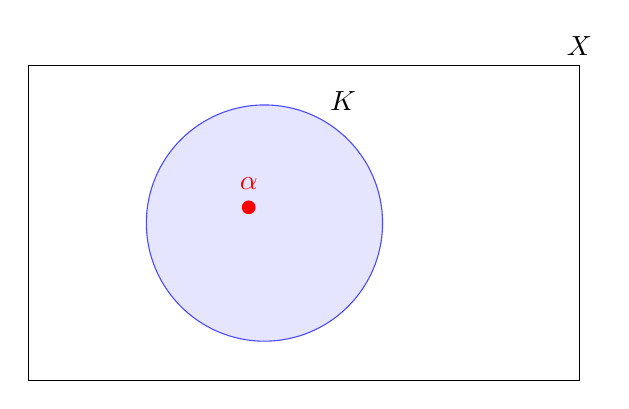
\begin{tikzpicture}
					\scope
					\clip (-4,-1) rectangle (3, 3)
					(0, 0) circle (1);
					\endscope
					\draw (-4,-1) rectangle (3, 3) node [text=black,above] {$X$};
					\draw[color=blue!70, fill=blue!10](-1, 1) circle (1.5) (0, 2.3)  node [text=black,above] {$K$};
					\draw[red, fill=red] (-1.2, 1.2) circle (0.08) (-1.2, 1.3) node [above] {$\alpha$};
				\end{tikzpicture}
			\end{center}
			There are 2 ways to make this:
			\begin{itemize}
				\item Make $K$ and choose $\alpha$ from $K$
				\item Choose $\alpha$ from $X$ and make $K$ including $\alpha$
			\end{itemize}
			The first way is $_{n}\mathrm{C}_{k}\cdot{_{k}\mathrm{C}_{1}} = k\cdot{_{n}\mathrm{C}_{k}}$ (make $K$ be $_{n}\mathrm{C}_{k}$, choose $\alpha$ be $_{k}\mathrm{C}_{1}$).\\
			The second way is $_{n}\mathrm{C}_{1}\cdot{_{n - 1}\mathrm{C}_{k - 1}} = n\cdot{_{n - 1}\mathrm{C}_{k - 1}}$ (choose $\alpha$ be $_{n}\mathrm{C}_{1}$, make $K$ be $_{n - 1}\mathrm{C}_{k - 1}$).\\
			Therefore, $k\cdot{_{n}\mathrm{C}_{k}} = n\cdot{_{n - 1}\mathrm{C}_{k - 1}}$.\\
			{\color{orange} \textbf{WARNING}}: This method is called \textit{combinatorial argument}. You {\color{red} \textbf{MUST}} tell the story in {\color{teal} \textbf{sentences}}, not in figures. Figures are not necessary, just for supporting purposes only. Drawing is not a logical explanation. If you only draw figures and do not write specific sentences, then you may get close to 0 points.\\
			{\color{cyan}\textbf{APPENDIX}}: The \textit{algebraic argument} is just calculate directly like following:
			\begin{align*}
				& k\cdot{_{n}\mathrm{C}_{k}}\\
				=\ & k\cdot\frac{n!}{k!(n - k)!}\\
				=\ & \frac{n!}{(k - 1)!(n - k)!}\\
				=\ & n\cdot\frac{(n - 1)!}{(k - 1)!(n - k)!}\\
				=\ & n\cdot\frac{(n - 1)!}{(k - 1)!(n - k)!}\\
				=\ & n\cdot\frac{(n - 1)!}{(k - 1)!(n - 1 - (k - 1))!}\\
				=\ & n\cdot{_{n - 1}\mathrm{C}_{k - 1}}
			\end{align*}
		\end{proof}
		\item \begin{proof}
			Consider the below situation:
			\begin{itemize}
				\item [] Let $X$ be a set with $|X| = n$. Make a new subset of $X$ with $r$ elements, let the subset be $R$. Make a new subset of $R$ with $k$ elements, let it be $K$.
			\end{itemize}
			\begin{center}
				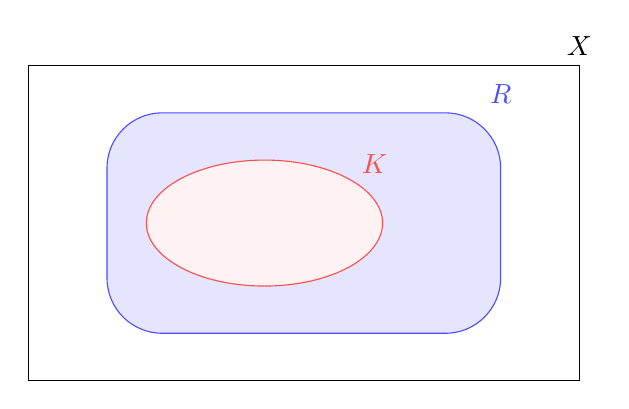
\begin{tikzpicture}
					\scope
					\clip (-4,-1) rectangle (3, 3)
					(0, 0) circle (1);
					\endscope
					\draw (-4,-1) rectangle (3, 3) node [text=black,above] {$X$};
					\draw[rounded corners=20, color=blue!70, fill=blue!10] (-3, -0.4) rectangle (2, 2.4)  node [above] {$R$};
					\draw[color=red!70, fill=red!5] (-1, 1) ellipse (1.5 and 0.8) (0.4, 1.5) node [above] {$K$};
				\end{tikzpicture}
			\end{center}
			There are 2 ways to make this:
			\begin{itemize}
				\item Make $R$ from $X$ and make $K$ from $R$
				\item Make $K$ from $X$ and make $R$ including $K$
			\end{itemize}
			The first way is $_{n}\mathrm{C}_{r}\cdot{_{r}\mathrm{C}_{k}}$ (make $R$ be $_{n}\mathrm{C}_{r}$, make $K$ be $_{r}\mathrm{C}_{k}$).\\
			The second way is $_{n}\mathrm{C}_{k}\cdot{_{n - k}\mathrm{C}_{r - k}}$ (make $K$ be $_{n}\mathrm{C}_{k}$, make $R$ be $_{n - k}\mathrm{C}_{r - k}$).\\
			Therefore, $_{n}\mathrm{C}_{r}\cdot{_{r}\mathrm{C}_{k}} = {_{n}\mathrm{C}_{k}}\cdot{_{n - k}\mathrm{C}_{r - k}}$.\\
		\end{proof}
		\item \begin{proof}
			Consider the below situation:
			\begin{itemize}
				\item [] Let $X$ be a set with $|X| = 2n$. There are 2 subsets of $X$: $A$ and $B$. They satisfy $|A| = n, |B| = n, A\cap B = \emptyset$. Make a new subset of X with $n$ elements, let the subset be $K$. Choose one element in $A\cap K$, let it be $\alpha$.
			\end{itemize}
			\begin{center}
				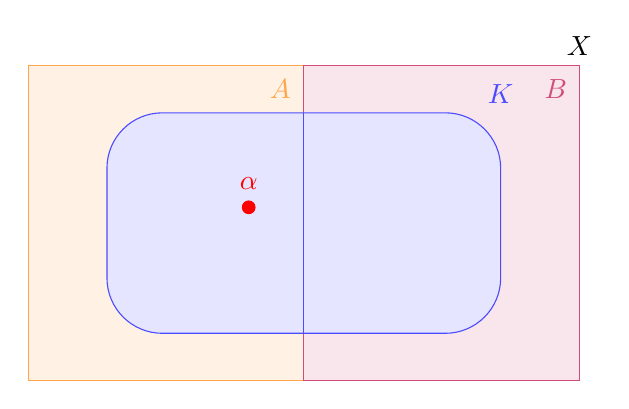
\begin{tikzpicture}
					\scope
					\clip (-4,-1) rectangle (3, 3)
					(0, 0) circle (1);
					\endscope
					\draw (-4,-1) rectangle (3, 3) node [text=black,above] {$X$};
					\draw[color=orange!70, fill=orange!10] (-4, -1) rectangle (-0.5, 3) (-0.8, 2.7) node {$A$};
					\draw[color=purple!70, fill=purple!10] (-0.5, -1) rectangle (3, 3) (2.7, 2.7) node {$B$};
					\draw[rounded corners=20, color=blue!70, fill=blue!10] (-3, -0.4) rectangle (2, 2.4)  node [above] {$K$};
					\draw[color=blue!70] (-0.5, -0.4) -- (-0.5, 2.4);
					\draw[red, fill=red] (-1.2, 1.2) circle (0.08) (-1.2, 1.3) node [above] {$\alpha$};
				\end{tikzpicture}
			\end{center}
			There are 2 ways to make this:
			\begin{itemize}
				\item Make $K$ from $X$(Choose from $A$ and $B$ each) and choose $\alpha$ from $A\cap K$
				\item Choose $\alpha$ from $A$ and make $K$ from $X$ including $\alpha$ 
			\end{itemize}
			Consider the first way. if you choose $k$ elements from $A$, then you can choose $n - k$ elements in $B$. This gives ${_{n}\mathrm{C}_{k}}\cdot{_{n}\mathrm{C}_{n - k}} = \left({_{n}\mathrm{C}_{k}}\right)^2$. This is true for $1 \leq k \leq n$. Note that $k = 0$ is impossible because we need to choose $\alpha$ in $A$. Choose $\alpha$ gives $_{k}\mathrm{C}_{1} = k$. From here, we get $\sum\limits_{k=1}^n k\left({_{n}\mathrm{C}_{k}}\right)^2$.\\
			The second way is $_{n}\mathrm{C}_{1}\cdot{_{2n - 1}\mathrm{C}_{n - 1}} = n\cdot{_{2n - 1}\mathrm{C}_{n - 1}}$ (choose $\alpha$ be $_{n}\mathrm{C}_{1}$, make $K$ be $_{2n - 1}\mathrm{C}_{n - 1}$).\\
			Therefore, $\sum\limits_{k=1}^n k\left(_{n}\mathrm{C}_{k}\right)^2 = n\cdot{_{2n - 1}\mathrm{C}_{n - 1}}$.\\
		\end{proof}
	\end{enumerate}